\documentclass[../main-sheet.tex]{subfiles}
\usepackage{../style}
\usepackage{cancel}
\graphicspath{ {../img/} }
\backgroundsetup{contents={}}
\begin{document}
Mode of this problem
\begin{align*}
    \text{Maximize }   & Z=x_1+4x_2 \quad \text{(objective function)}                               \\
    \text{Subject to } &
    \begin{aligned}
        \begin{rcases}
            6x_1+4x_2 \leq 24 \\
            x_1+2x_2 \leq 6   \\
            -x_1+x_2 \leq 1   \\
            x_2 \leq 2
        \end{rcases}
    \end{aligned}
    \text{Constraints (or, Restriction)}                                                            \\
                       & x_1,x_2\geq 0 \quad \text{Non-negativity restriction on decision variable}
\end{align*}

$$
\begin{array}{r}
  \text{Maximize } \quad Z=5 x_{1}+4 x_{2} \quad\text{(objective function)\qquad}\\
\end{array}$$ $$
\left.\begin{array}{r}
    \text{Subject to} \quad 
    6 x_{1}+4 x_{2} \leq 24 \\
    x_{1}+2 x_{2} \leq 6    \\
    -x_{1}+x_{2} \leq 1     \\
    x_{2} \leq 2            \\
\end{array}\right\} \text { Constraints (or, Restriction) }
$$
\[
    \begin{array}{l}
        \hspace{0.5em}\text{Maximize } \quad Z=5 x_{1}+4 x_{2} \quad\text{(objective function)\qquad}\\
        \left.\begin{array}{r}
            \text{Subject to} \quad
            6 x_{1}+4 x_{2} \leq 24 \\
            x_{1}+2 x_{2} \leq 6    \\
            -x_{1}+x_{2} \leq 1     \\
            x_{2} \leq 2            \\
        \end{array}\right\} \text { Constraints (or, Restriction) }\\
        \begin{array}{r}
            \qquad \qquad \qquad \qquad \quad x_1,x_2\geq 0 \quad \text{Non-negativity restriction on decision variable}\\
        \end{array}
    \end{array}
\]

% Table generated by Excel2LaTeX from sheet 'Sheet1'
% Table generated by Excel2LaTeX from sheet 'Sheet1'
\begin{table}[htbp]
    \begin{tabular}{ccccccccc}
    \toprule
     &  &  & 3 & 2 & 0 & 0 & 0 &Constant/  \\ \cmidrule(lr){4-8}
    \multirow{-2}{*}{Tab} & \multirow{-2}{*}{\(C_B\)} & \multirow{-2}{*}{\diagbox{basis}{\(c_j \to\)}} & \(x_1\) & \(x_2\) & \(S_1\) & \(S_2\) & \(S_3\) & Solution \\ \midrule
     & 0 & \(S_1\) & \cellcolor[HTML]{FFCCC9}-1 & 2 & 1 & 0 & 0 & 4 \\
     & 0 & \(S_2\) & \cellcolor[HTML]{FFCCC9}3 & 2 & 0 & 1 & 0 & 14 \\
     & 0 & \(S_3\) & \cellcolor[HTML]{96FFFB}1 & \cellcolor[HTML]{9AFF99}-1 & \cellcolor[HTML]{9AFF99}0 & \cellcolor[HTML]{9AFF99}0 & \cellcolor[HTML]{9AFF99}1 & 3 \\ \cmidrule(l){2-9} 
    \multirow{-4}{*}{I} & \multicolumn{2}{c}{\(c_j\) row} & 3 & 2 & 0 & 0 & 0 & Z=0 \\ \midrule
     & 0 & \(S_1\) & 0 & \cellcolor[HTML]{FFCCC9}1 & 1 & 0 & 1 & 7 \\
     & 0 & \(S_2\) & \cellcolor[HTML]{9AFF99}0 & \cellcolor[HTML]{96FFFB}5 & \cellcolor[HTML]{9AFF99}0 & \cellcolor[HTML]{9AFF99}1 & \cellcolor[HTML]{9AFF99}-3 & 5 \\
     & 3 & \(x_1\) & 1 & \cellcolor[HTML]{FFCCC9}-1 & 0 & 0 & 1 & 3 \\ \cmidrule(l){2-9} 
    \multirow{-4}{*}{II} & \multicolumn{2}{c}{\(c_j\) row} & 0 & 5 & 0 & 0 & -3 & Z=9 \\ \midrule
     & 0 & \(S_1\) & \cellcolor[HTML]{9AFF99}0 & \cellcolor[HTML]{9AFF99}0 & \cellcolor[HTML]{9AFF99}1 & \cellcolor[HTML]{9AFF99}-1/5 & \cellcolor[HTML]{96FFFB}8/5 & 6 \\
     & 2 & \(x_2\) & 0 & 1 & 0 & 1/5 & \cellcolor[HTML]{FFCCC9}-3/5 & 1 \\
     & 3 & \(x_1\) & 1 & 0 & 0 & 1/5 & \cellcolor[HTML]{FFCCC9}2/5 & 4 \\ \cmidrule(l){2-9} 
    \multirow{-4}{*}{III} & \multicolumn{2}{c}{\(c_j\) row} & 0 & 0 & 0 & -1 & 0 & Z=14 \\ \midrule
     & 0 & \(S_1\) & 0 & 0 & 5/8 & -1/8 & 1 & 15/4 \\
     & 2 & \(x_2\) & 0 & 1 & 3/8 & 1/8 & 0 & 13/4 \\
     & 3 & \(x_1\) & 1 & 0 & -1/4 & 1/4 & 0 & 5/2 \\ \cmidrule(l){2-9} 
    \multirow{-4}{*}{IV} & \multicolumn{2}{c}{\(c_j\) row} & 0 & 0 & 0 & -1 & 0 & Z=14 \\ \bottomrule
    \end{tabular}
    \end{table}
    \begin{align*}
        \max/\min              &\; Z= c_{1}x_{1} + c_{2}x_{2}+\dots + c_nx_n \\
        \text{subject to} &\;
        \begin{alignedat}[t]{5}
        a_{11}x_{1}&+{} &a_{12}x_{2}& +{} &\dots& +{} &a_{1n}x_n (& \leq or & = or & \geq) b_{1} \\
        a_{21}x_{1}&+{} &a_{22}x_{2}& +{} &\dots& +{} &a_{2n}x_n (& \leq or & = or & \geq) b_{2} \\
               \dots & &        \dots&  && \dots &          &         &         \dots &\\
        a_{m1}x_{1}&+{} &a_{m2}x_{2}& +{} &\dots& +{} &   a_{mn}x_n (& \leq or & = or &    \geq) b_m \\
                 & &           &     &   &     &          &         &      x_j&  \geq0(j=1,2,\dots,n)
        \end{alignedat}
        \end{align*}
        \begin{align*}
            \max/\min              &\; Z=\sum_{j=1}^n c_j x_j \\
            \text{subject to} &\;
            \begin{alignedat}[t]{3}
            \sum a_{ij}x_{j}& (\leq or & = or& \geq) b_i(i=1,2,m) \\
                           &  &                 x_j &\geq0(j=1,2,...n)
            \end{alignedat}
            \end{align*}

            \newpage
\begin{table}[H]
\centering
\begin{tabular}{ccccccccc}
% \toprule
 &  &  & 3 & 2 & 0 & 0 & 0 &Constant/  \\ \cmidrule(lr){4-8}
\multirow{-2}{*}{Tab} & \multirow{-2}{*}{\(c_B\)} & \multirow{-2}{*}{\diagbox{basis}{\(c_j \to\)}} & \(x_1\) & \(x_2\) & \(S_1\) & \(S_2\) & \(S_3\) & Solution \\ \midrule
 & 0 & \(S_1\) & \cellcolor[HTML]{FFCCC9}-1 & 2 & 1 & 0 & 0 & 4 \\
 & 0 & \(S_2\) & \cellcolor[HTML]{FFCCC9}3 & 2 & 0 & 1 & 0 & 14 \\
 & 0 & \(S_3\) & \cellcolor[HTML]{96FFFB}1 & \cellcolor[HTML]{9AFF99}-1 & \cellcolor[HTML]{9AFF99}0 & \cellcolor[HTML]{9AFF99}0 & \cellcolor[HTML]{9AFF99}1 & 3 \\ \cmidrule(l){2-9} 
\multirow{-4}{*}{I} & \multicolumn{2}{c}{\(\bar{c_j}\) row} & 3 & 2 & 0 & 0 & 0 & Z=0 \\ \midrule
 & 0 & \(S_1\) & 0 & \cellcolor[HTML]{FFCCC9}1 & 1 & 0 & 1 & 7 \\
 & 0 & \(S_2\) & \cellcolor[HTML]{9AFF99}0 & \cellcolor[HTML]{96FFFB}5 & \cellcolor[HTML]{9AFF99}0 & \cellcolor[HTML]{9AFF99}1 & \cellcolor[HTML]{9AFF99}-3 & 5 \\
 & 3 & \(x_1\) & 1 & \cellcolor[HTML]{FFCCC9}-1 & 0 & 0 & 1 & 3 \\ \cmidrule(l){2-9} 
\multirow{-4}{*}{II} & \multicolumn{2}{c}{\(\bar{c_j}\) row} & 0 & 5 & 0 & 0 & -3 & Z=9 \\ \midrule
 & 0 & \(S_1\) & \cellcolor[HTML]{9AFF99}0 & \cellcolor[HTML]{9AFF99}0 & \cellcolor[HTML]{9AFF99}1 & \cellcolor[HTML]{9AFF99}-1/5 & \cellcolor[HTML]{96FFFB}8/5 & 6 \\
 & 2 & \(x_2\) & 0 & 1 & 0 & 1/5 & \cellcolor[HTML]{FFCCC9}-3/5 & 1 \\
 & 3 & \(x_1\) & 1 & 0 & 0 & 1/5 & \cellcolor[HTML]{FFCCC9}2/5 & 4 \\ \cmidrule(l){2-9} 
\multirow{-4}{*}{III} & \multicolumn{2}{c}{\(\bar{c_j}\) row} & 0 & 0 & 0 & -1 & 0 & Z=14 \\ \midrule
 & 0 & \(S_1\) & 0 & 0 & 5/8 & -1/8 & 1 & 15/4 \\
 & 2 & \(x_2\) & 0 & 1 & 3/8 & 1/8 & 0 & 13/4 \\
 & 3 & \(x_1\) & 1 & 0 & -1/4 & 1/4 & 0 & 5/2 \\ \cmidrule(l){2-9} 
\multirow{-4}{*}{IV} & \multicolumn{2}{c}{\(\bar{c_j}\) row} & 0 & 0 & 0 & -1 & 0 & Z=14 \\ \bottomrule
\end{tabular}
\end{table}
\begin{table}[H]
    \centering
    \begin{tabular}{cccccccccc}
        % \toprule
                                &                            &                                                & 5                                      & 4                                       & 0                                        & 0                                     & 0                                     & 0                                     & Constant/ \\ \cmidrule(lr){4-9}
        \multirow{-2}{*}{Tab}   & \multirow{-2}{*}{\(c_B\)}  & \multirow{-2}{*}{\diagbox{basis}{\(c_j \to\)}} & \(x_1\)                                & \(x_2\)                                 & \(S_1\)                                  & \(S_2\)                               & \(S_3\)                               & \(S_4\)                               & Solution  \\ \midrule
        \multirow{5}[3]{*}{I} & 0     & $ S_1 $ & \cellcolor[rgb]{ .588,  1,  .984}6 & \cellcolor[rgb]{ .604,  1,  .6}4 & \cellcolor[rgb]{ .604,  1,  .6}1 & \cellcolor[rgb]{ .604,  1,  .6}0 & \cellcolor[rgb]{ .604,  1,  .6}0 & \cellcolor[rgb]{ .604,  1,  .6}0 & 24 \\
        & 0     & $ S_2 $ & \cellcolor[rgb]{ 1,  .8,  .788}1 & 2     & 0     & 1     & 0     & 0     & 6 \\
        & 0     & $ S_3 $ & \cellcolor[rgb]{ 1,  .8,  .788}-1 & 1     & 0     & 0     & 1     & 0     & 1 \\
        & 0     & $ S_4 $ & \cellcolor[rgb]{ 1,  .8,  .788}0 & 1     & 0     & 0     & 0     & 1     & 2 \\
\cmidrule{2-10}          & \multicolumn{2}{c}{$ \bar{c_j} $ row} & 5     & 4     & 0     & 0     & 0     & 0     & Z=0 \\
  \midrule
  \multirow{5}[4]{*}{II} & 5     & $x_1$ & 1     & \cellcolor[rgb]{ 1,  .8,  .788}2/3 & 1/6   & 0     & 0     & 0     & 4 \\
        & 0     & $S_2$ & \cellcolor[rgb]{ .604,  1,  .6}0 & \cellcolor[rgb]{ .588,  1,  .984}4/3 & \cellcolor[rgb]{ .604,  1,  .6}-1/6 & \cellcolor[rgb]{ .604,  1,  .6}1 & \cellcolor[rgb]{ .604,  1,  .6}0 & \cellcolor[rgb]{ .604,  1,  .6}0 & 2 \\
        & 0     & $S_3$ & 0     & \cellcolor[rgb]{ 1,  .8,  .788}5/3 & 1/6   & 0     & 1     & 0     & 5 \\
        & 0     & $S_4$ & 0     & \cellcolor[rgb]{ 1,  .8,  .788}1 & 0     & 0     & 0     & 1     & 2 \\
\cmidrule{2-10}          & \multicolumn{2}{c}{$ \bar{c_j} $ row} & 0     & 2/3   & -5/6  & 0     & 0     & 0     & Z=20 \\
  \midrule
  \multirow{5}[4]{*}{III} & 5     & $x_1$ & 1     & 0     & 1/4   & 1/2   & 0     & 0     & 3 \\
        & 4     & $ x_2$ & 0     & 1     & -1/8  & 3/4   & 0     & 0     & 3/2 \\
        & 0     & $S_3$ & 0     & 0     & 3/8   & -5/4  & 1     & 0     & 5/2 \\
        & 0     & $S_4$ & 0     & 0     & 1/8   & -3/4  & 0     & 1     & 1/2 \\
\cmidrule{2-10}          & \multicolumn{2}{c}{$ \bar{c_j} $ row} & 0     & 0     & -3/4  & -11/2 & 0     & 0     & Z=21 \\
  \bottomrule

    \end{tabular}
\end{table}
\begin{table}[H]
    \centering
    % \begin{tabular}{p{5cm}p{5cm}}
    %     Primal & Dual\\
    %     {\begin{maxi*}
    %         {}{Z=3x_1+2x_2}{}{}
    %         \addConstraint{-x_1+2x_2}{\leq 4}
    %         \addConstraint{3x_1+2x_2}{\leq 14}
    %         \addConstraint{x_1-x_2}{\leq 3}
    %         \addConstraint{x_1,x_2}{\geq 0}
    %     \end{maxi*}} & {\begin{maxi*}
    %         {}{Z=3x_1+2x_2}{}{}
    %         \addConstraint{-x_1+2x_2}{\leq 4}
    %         \addConstraint{3x_1+2x_2}{\leq 14}
    %         \addConstraint{x_1-x_2}{\leq 3}
    %         \addConstraint{x_1,x_2}{\geq 0}
    %     \end{maxi*}}\\
    % \end{tabular}
    \begin{tabular}{ll}
        \multicolumn{1}{c}{PRimal} & \multicolumn{1}{c}{Dual} \\
        Minimize \(Z=12x_1+20x_2\) & Maximimize \(W=100y_1+120y_2\) \\
        subject to & subjeccy to \\
        \multicolumn{1}{r}{\(\begin{aligned}
             6x_1+8x_2&\geq 100\\
             7x_1+12x_2&\geq 120\\
             x_1,\,x_2&\geq 0
         \end{aligned}\)}&\multicolumn{1}{r}{\(\begin{aligned}
            6x_1+8x_2&\geq 100\\
             7x_1+12x_2&\geq 120\\
             x_1,\,x_2&\geq 0
        \end{aligned}\)}\\ 
        \end{tabular}
\end{table}
\newpage
\begin{table}[H]
    \begin{tabular}{l|ll|ll|ll|ll|l}
     & \multicolumn{2}{l|}{M1} & \multicolumn{2}{l|}{M2} & \multicolumn{2}{l|}{M3} & \multicolumn{2}{l|}{M4} &  \\ \hline
    \multicolumn{1}{c|}{\multirow{2}{*}{W1}} & 3 &  & 0 &  & 0 &  & 0 &  & \multirow{2}{*}{3} \\ \cline{3-3} \cline{5-5} \cline{7-7} \cline{9-9}
    \multicolumn{1}{c|}{} & \multicolumn{1}{l|}{} & 2 & \multicolumn{1}{l|}{} & 2 & \multicolumn{1}{l|}{} & 2 & \multicolumn{1}{l|}{} & 1 &  \\ \hline
    \multirow{2}{*}{W2} & 1 &  & 3 &  & 3 &  &  &  & 7 \\ \cline{3-3} \cline{5-5} \cline{7-7} \cline{9-9}
     & \multicolumn{1}{l|}{} & 10 & \multicolumn{1}{l|}{} & 8 & \multicolumn{1}{l|}{} & 5 & \multicolumn{1}{l|}{} & 4 &  \\ \hline
    \multirow{2}{*}{W3} &  &  &  &  & 1 &  & 4 &  & 5 \\ \cline{3-3} \cline{5-5} \cline{7-7} \cline{9-9}
     & \multicolumn{1}{l|}{} & 7 & \multicolumn{1}{l|}{} & 6 & \multicolumn{1}{l|}{} & 6 & \multicolumn{1}{l|}{} & 8 &  \\ \hline
    \end{tabular}
    \end{table}
    \newpage

    \def\Mc[#1]#2#3{\multicolumn{#1}{#2}{#3}}
\def\mc#1#2{\multicolumn{1}{#1}{#2}}

% \extrarowheight=6pt
\begin{tabular}{c|cc|cc|cc|cc|cc|c}
\mc{c}{}& \Mc[2]{c}{$M_1$} & \Mc[2]{c}{$M_2$} & \Mc[2]{c}{$M_3$} & Supply \\[6pt]\cline{2-11}
  1     & \mc{c|}{$x_{11}$} &&  \mc{c|}{$x_{12}$} && \mc{c|}{$\cdots$} && \mc{c|}{$\cdots$} && \mc{c|}{$x_{1n}$} && $a_1$\\[6pt]\cline{2-2}\cline{4-4}\cline{6-6}\cline{8-8}\cline{10-10}
        && \mc{c|}{$c_{11}$} && \mc{c|}{$c_{12}$} && \mc{c|}{$\cdots$} && \mc{c|}{$\cdots$} && \mc{c|}{$c_{1n}$} & \\[6pt]\cline{2-11}
  2     & \mc{c|}{$x_{21}$} &&  \mc{c|}{$x_{22}$} && \mc{c|}{$\cdots$} && \mc{c|}{$\cdots$} && \mc{c|}{$x_{2n}$} && $a_2$\\[6pt]\cline{2-2}\cline{4-4}\cline{6-6}\cline{8-8}\cline{10-10}
        && \mc{c|}{$c_{21}$} && \mc{c|}{$c_{22}$} && \mc{c|}{$\cdots$} && \mc{c|}{$\cdots$} && \mc{c|}{$c_{2n}$} & \\[6pt]\cline{2-11}
  3     & \mc{c|}{$\cdots$} &&  \mc{c|}{$\cdots$} && \mc{c|}{$\cdots$} && \mc{c|}{$\cdots$} && \mc{c|}{$\cdots$} && $a_3$\\[6pt]\cline{2-2}\cline{4-4}\cline{6-6}\cline{8-8}\cline{10-10}
        && \mc{c|}{$\cdots$} && \mc{c|}{$\cdots$} && \mc{c|}{$\cdots$} && \mc{c|}{$\cdots$} && \mc{c|}{$\cdots$} & \\[6pt]\cline{2-11}
$\cdot$ & \mc{c|}{$\cdots$} &&  \mc{c|}{$\cdots$} && \mc{c|}{$\cdots$} && \mc{c|}{$\cdots$} && \mc{c|}{$\cdots$} && $\cdot$\\[6pt]\cline{2-2}\cline{4-4}\cline{6-6}\cline{8-8}\cline{10-10}
$\cdot$ && \mc{c|}{$\cdots$} && \mc{c|}{$\cdots$} && \mc{c|}{$\cdots$} && \mc{c|}{$\cdots$} && \mc{c|}{$\cdots$} &  $\cdot$\\[6pt]\cline{2-11}
$\cdot$ & \mc{c|}{$x_{m1}$} &&  \mc{c|}{$x_{m2}$} && \mc{c|}{$\cdots$} && \mc{c|}{$\cdots$} && \mc{c|}{$x_{mn}$} && $\cdot$\\[6pt]\cline{2-2}\cline{4-4}\cline{6-6}\cline{8-8}\cline{10-10}
$m$     && \mc{c|}{$c_{m1}$} && \mc{c|}{$x_{m2}$} && \mc{c|}{$\cdots$} && \mc{c|}{$\cdots$} && \mc{c|}{$c_{mn}$} & $a_{m}$\\[6pt]\cline{2-11}
\mc{c}{Demand}& \Mc[2]{c}{$b_1$} & \Mc[2]{c}{$b_2$} & \Mc[2]{c}{$\cdots$} & \Mc[2]{c}{$\cdots$} & \Mc[2]{c}{$b_n$} &  \\
\end{tabular}\newpage
\begin{table}[H]
    \begin{tabular}{|c|cc|cc|cc|cc|c|}
    \hline
     & \multicolumn{2}{c|}{$M_1$} & \multicolumn{2}{c|}{$M_2$} & \multicolumn{2}{c|}{$M_3$} & \multicolumn{2}{c|}{$M_4$} & Supply \\ \hline
    \multicolumn{1}{|c|}{\multirow{2}{*}{W1}} & 3 &  &  &  &  &  &  &  & \multirow{2}{*}{$\cancel{3}$} \\ \cline{3-3} \cline{5-5} \cline{7-7} \cline{9-9}
    \multicolumn{1}{|c|}{} & \multicolumn{1}{l|}{} & 2 & \multicolumn{1}{l|}{} & 2 & \multicolumn{1}{l|}{} & 2 & \multicolumn{1}{l|}{} & 1 &  \\ \hline
    \multirow{2}{*}{W2} & 1 &  & 3 &  & 3 &  &  &  & \multirow{2}{*}{\cancel{7} \cancel{6} \cancel{3}} \\ \cline{3-3} \cline{5-5} \cline{7-7} \cline{9-9}
     & \multicolumn{1}{l|}{} & 10 & \multicolumn{1}{l|}{} & 8 & \multicolumn{1}{l|}{} & 5 & \multicolumn{1}{l|}{} & 4 &  \\ \hline
    \multirow{2}{*}{W3} &  &  &  &  & 1 &  & 4 &  & \multirow{2}{*}{5} \\ \cline{3-3} \cline{5-5} \cline{7-7} \cline{9-9}
     & \multicolumn{1}{l|}{} & 7 & \multicolumn{1}{l|}{} & 6 & \multicolumn{1}{l|}{} & 6 & \multicolumn{1}{l|}{} & 8 &  \\ \hline
    Demand & \multicolumn{2}{l|}{4} & \multicolumn{2}{l|}{3} & \multicolumn{2}{l|}{4} & \multicolumn{2}{l|}{4} &  \\ \hline
    \end{tabular}
    \end{table}
    \newpage
    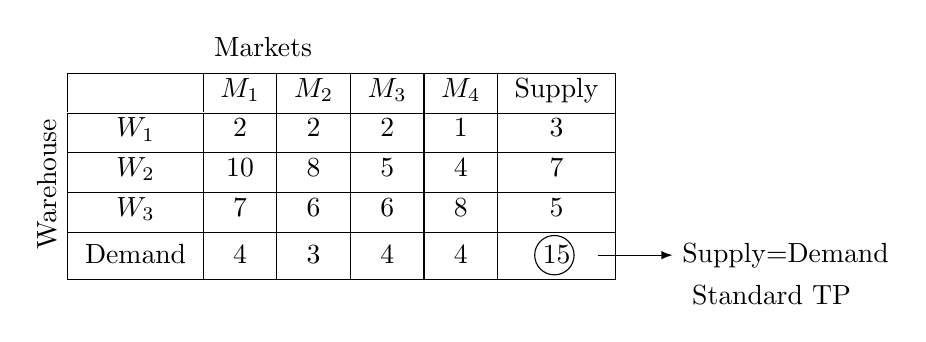
\begin{tikzpicture}
        % \extrarowheight=6pt
        %     \matrix[ampersand replacement=\&] {
        %         \node {
        %             \begin{tabular}{|c| c| c|}
        %             \hline
        %                 1&2&3\\
        %                 \hline
        %                 1&2&3\\
        %                 \hline
        %                 1&2&3\\
        %                 \hline
        %             \end{tabular}
        %         };
        %         \& 
        %         \node {b}; \\
        %         \node {c}; \& \node {d}; \\
        % };
        % \draw (0,0) grid (10,10);
        % \node at (0.5,0.5) {Demand};
        \node at (0,0) {
            \begin{tabular}[t]{|c|c|c|c|c|c|}
                \hline 
                   & $M_1$ & $M_2$ & $M_3$ & $M_4$ & Supply  \\[2pt] 
                   \hline
                $W_1$   & 2    & 2    & 2    & 1    & 3      \\[2pt] \hline
                $W_2$   & 10   & 8    & 5    & 4    & 7      \\[2pt] \hline
                $W_3$   & 7    & 6    & 6    & 8    & 5      \\[2pt] \hline
                \rule{0pt}{11pt}Demand & 4    & 3    & 4    & 4    & 15     \\[2pt] \hline
            \end{tabular}
        };
        \node at (-1,1.65) {Markets};
        \node [rotate=90] at (-3.75,-.1) {Warehouse};
        \draw (2.7,-1) circle (.25);
        \draw[-latex](3.25,-1)--(4.2,-1)node[right]{Supply=Demand};
        \node at (5.4,-1.5) {$\therefore$ Standard TP};
        \end{tikzpicture}
\end{document}